\documentclass[../main.tex]{subfiles}
\begin{document}

\section{Combining Pose Estimation with Pick and Place Execution} \label{sec:combination}
In this section, a combination of the developed pose estimation method and robot motion planning method is described.

Based on the results in section \ref{subsubsec:comparision_robotics}, the robot motion planning method: point to point interpolation with parabolic blend, was deemed most suitable for this task. This is because the method has some predefined points, which are constructed so that the robot avoids singularities. Even though the Rapidly-exploring Random Trees Connect method calculated a shorter path, the path was generated randomly which could potentially lead the robot close to singularities.

Based on the results in section \ref{subsec:vision_comparison}, the simulated depth sensor method is integrated into the combined system. The simulated depth sensor showed the most precise results when considering rotation and position error. 

The pipeline for the combination is illustrated in figure \ref{fig:combi_pipeline}.
\begin{figure}[H]
    \centering
    \noindent\makebox[\textwidth][c]{\subfile{figures/combi/pipeline}}
    \caption{Illustration of the pipeline for the combination of pose estimation and pick and place execution.}
    \label{fig:combi_pipeline}
\end{figure}

In Figure \ref{subfig:duck_axis}, the coordinate frame for the object to be picked is shown. The z-axis of the object frame points in the opposite direction to the TCP, thus when calculating the configuration of the estimated pose it is rotated $180$ degrees around the x-axis. Furthermore, the coordinate frame of the object is at the bottom, thereby the TCP comes in collision with the object when trying to grasp it. Therefore, the z position is adjusted so the TCP does not collide with the object when grasping is performed. The grasp target coordinate frame is shown in figure \ref{subfig:grasp_target_axis}, which makes the robot able to grasp the object as shown in figure \ref{subfig:grasped_object}. The object used is the duck \cite{rubber_duck} that is also used in Section \ref{sec:vision} for the pose estimation.
\begin{figure}[H]
    \centering
    \begin{subfigure}[t]{0.3\textwidth}
        \centering
        \captionsetup{width=0.9\textwidth}
        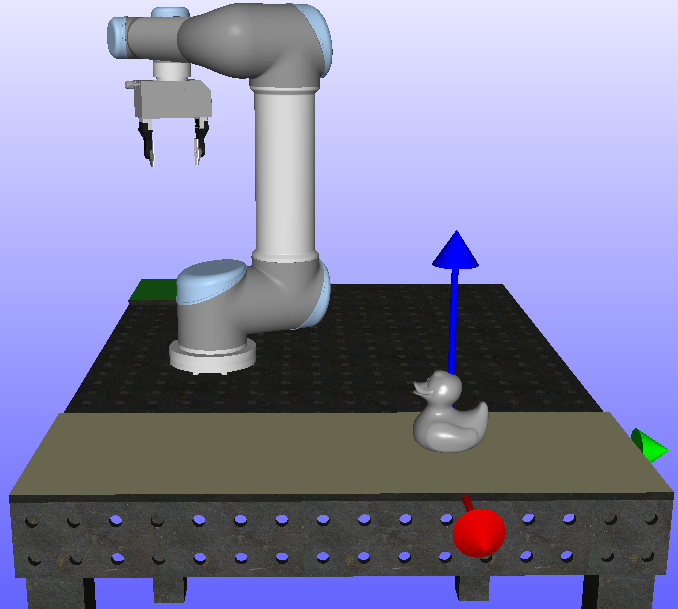
\includegraphics[width=0.9\textwidth]{figures/combi/duck_axis.png}
        \caption{The coordinate frame for the object.}
        \label{subfig:duck_axis}
    \end{subfigure}
    \begin{subfigure}[t]{0.275\textwidth}
        \centering
        \captionsetup{width=0.9\textwidth}
        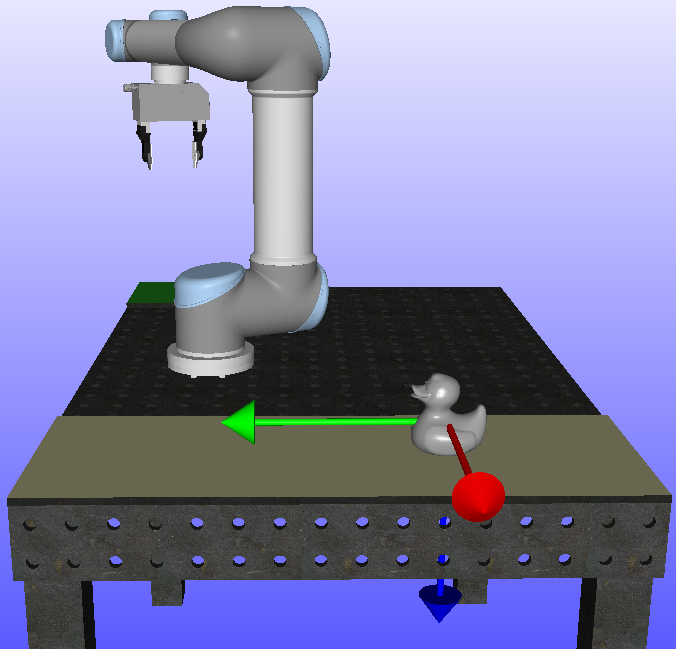
\includegraphics[width=0.9\textwidth]{figures/combi/grasp_target_axis.png}
        \caption{The coordinate frame for the grasp target of object.}
        \label{subfig:grasp_target_axis}
    \end{subfigure}
    \begin{subfigure}[t]{0.33\textwidth}
        \centering
        \captionsetup{width=0.9\textwidth}
        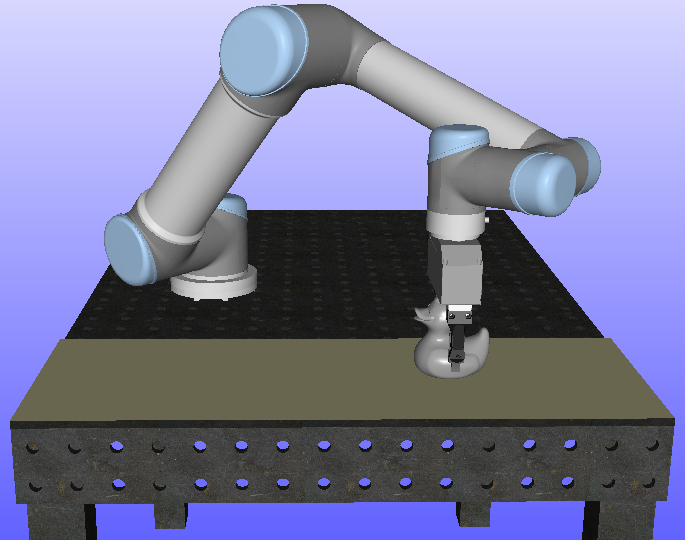
\includegraphics[width=0.9\textwidth]{figures/combi/grasped_object.png}
        \caption{The robot grasping the object.}
        \label{subfig:grasped_object}
    \end{subfigure}
    \caption{Illustration of how the object is grasped.}
    \label{fig:grasping_object}
\end{figure}
A video of the combined pose estimation and pick and place can be seen at \cite{combi_vid}, which shows the task completed at three different object locations.

\end{document}